% !TeX program = lualatex
% !TeX encoding = UTF-8
% !TeX spellcheck = pt_BR

\documentclass[12pt,a4paper]{article}

\usepackage{fontspec}
\defaultfontfeatures{Ligatures=TeX}
\setmainfont{Latin Modern Roman}
\setsansfont{Latin Modern Sans}
\setmonofont{Latin Modern Mono}
\usepackage[brazilian]{babel}
\usepackage{geometry}
\geometry{top=2.2cm,bottom=2.2cm,left=2.1cm,right=2.1cm}
\usepackage{microtype}
\usepackage{graphicx}
\usepackage{booktabs}
\usepackage{tabularx}
\usepackage{array}
\usepackage{enumitem}
\usepackage{xcolor}
\usepackage{listings}
\usepackage{tikz}
\usetikzlibrary{arrows.meta,positioning}
\usepackage{xurl}
\usepackage{hyperref}
\usepackage{fancyhdr}
\usepackage{lastpage}

\definecolor{primary}{HTML}{1D4ED8}
\definecolor{accent}{HTML}{166534}
\definecolor{warning}{HTML}{B91C1C}
\definecolor{codegray}{HTML}{F3F4F6}
\definecolor{rulegray}{HTML}{D1D5DB}
\hypersetup{
  colorlinks=true,linkcolor=primary,urlcolor=primary,
  pdfauthor={Sergio Cordero Calvimontes},
  pdftitle={Relatório técnico — 2D Plotter},
  pdfsubject={Controle cartesiano com Arduino Uno e Wokwi}
}

\pagestyle{fancy}
\fancyhf{}
\lhead{2D Plotter}
\rhead{Relatório técnico}
\cfoot{Página \thepage\ de \pageref{LastPage}}
\setlength{\headheight}{14.5pt}
\setlength{\parindent}{1.1cm}
\setlength{\parskip}{0.2em}
\setlength{\emergencystretch}{2em}
\setlist{itemsep=0.25em,topsep=0.4em}
\newcolumntype{Y}{>{\raggedright\arraybackslash}X}

\lstdefinestyle{cppstyle}{
  language=C++,basicstyle=\small\ttfamily,backgroundcolor=\color{codegray},
  frame=single,rulecolor=\color{rulegray},numbers=left,
  numberstyle=\scriptsize\color{gray},keywordstyle=\color{primary}\bfseries,
  commentstyle=\color{accent},stringstyle=\color{warning},
  showstringspaces=false,breaklines=true,columns=fullflexible
}
\lstset{style=cppstyle}

\newcommand{\WokwiURL}{https://wokwi.com/projects/472168224663835649}
\newcommand{\GitHubURL}{https://github.com/Argus-Kepheus/2d-plotter}
\newcommand{\CandidateName}{Sergio Cordero Calvimontes}

\begin{document}

\begin{titlepage}
  \centering
  \vspace*{0.6cm}
  {\Large Projeto de automação e controle\par}
  \vspace{0.9cm}
  {\Huge\bfseries 2D Plotter\par}
  \vspace{0.35cm}
  {\Large Controle cartesiano com Arduino Uno e Wokwi\par}
  \vspace{0.8cm}
  \href{\GitHubURL}{%
    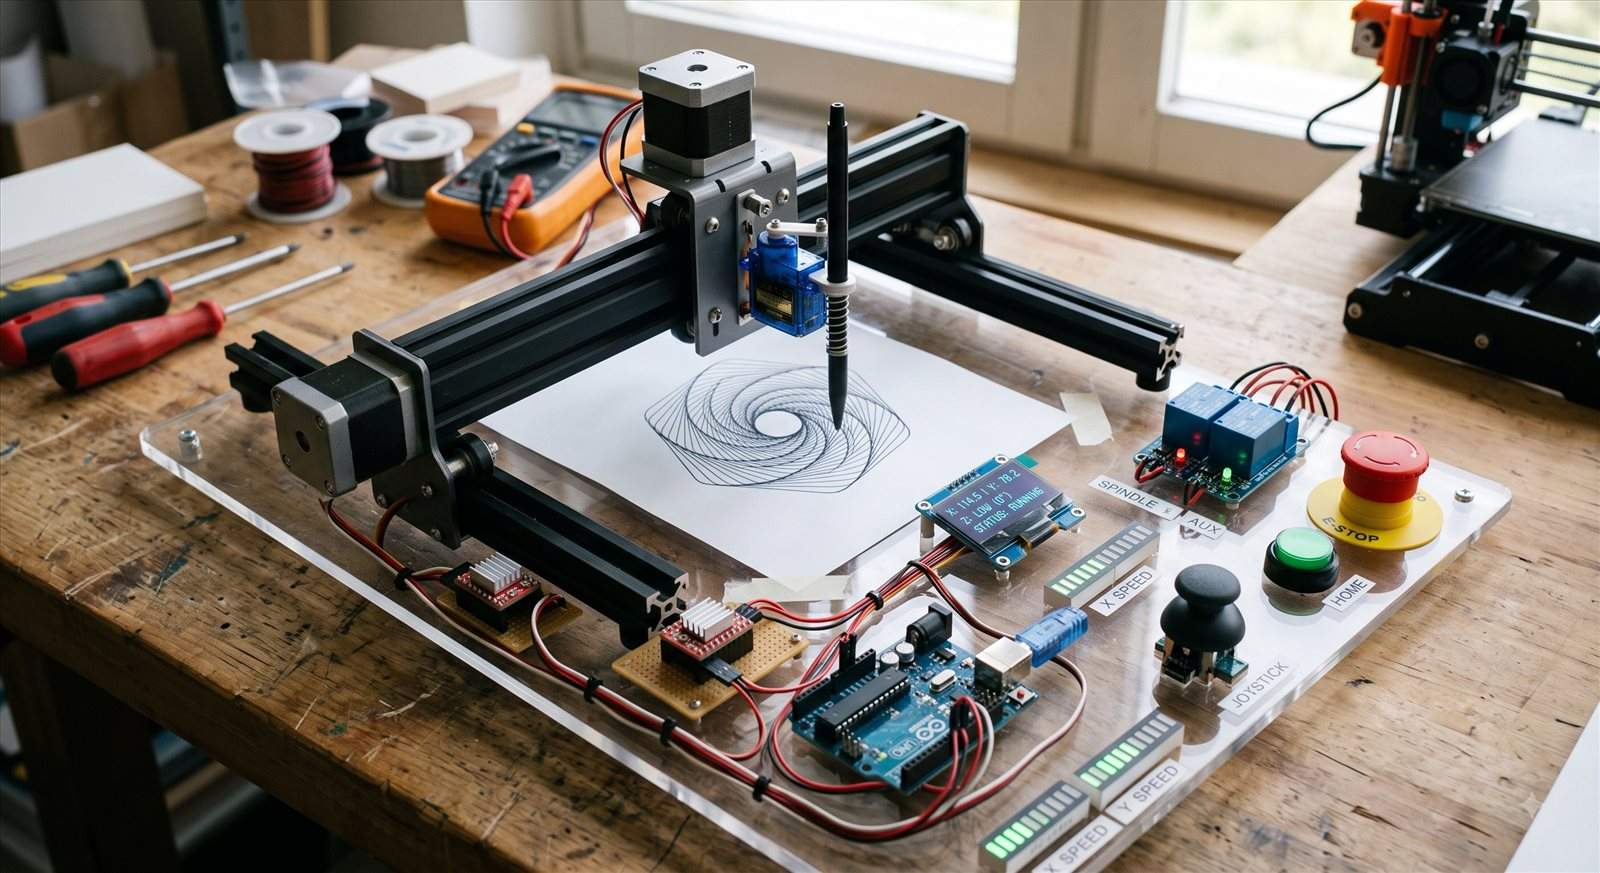
\includegraphics[
      width=\textwidth,
      height=0.40\textheight,
      keepaspectratio
    ]{figures/front-cover.png}%
  }\par
  \vspace{0.2cm}
  {\small\itshape Ilustração conceitual do sistema; clique para acessar o repositório.\par}
  \vspace{0.7cm}
  \begin{tabular}{rl}
    Responsável: & \CandidateName \\
    Plataforma: & Arduino Uno R3 \\
    Linguagem: & Arduino C++ \\
    Simulação: & Wokwi
  \end{tabular}
  \vfill
  {\large \today\par}
\end{titlepage}

\tableofcontents
\newpage

\section{Introdução}

Este projeto desenvolve o controle simulado de uma plotter cartesiana de dois
eixos. O sistema reúne acionamento de motores de passo, posicionamento da
caneta, interação por joystick, telemetria, sinalização de velocidade, cargas
auxiliares e funções de parada. A simulação executável está disponível em
\url{\WokwiURL}; os arquivos \texttt{sketch.ino}, \texttt{diagram.json} e
\texttt{libraries.txt} tornam a implementação reproduzível.

Além do funcionamento, a organização do repositório separa fontes,
documentação bilíngue, verificações e artefatos de relatório. Essa separação
facilita auditoria entre requisitos, pinagem, diagrama e firmware.

\section{Objetivos e requisitos}

O objetivo principal é comandar os eixos X/Y com movimento acelerado e limites
lógicos, enquanto a caneta assume três alturas. Como requisitos complementares,
o sistema deve apresentar a posição em OLED, indicar a velocidade dos eixos,
controlar sucção e ventilação e reagir imediatamente ao E-STOP.

\begin{table}[htbp]
  \centering
  \caption{Principais parâmetros do projeto.}
  \begin{tabularx}{\textwidth}{@{}YY@{}}
    \toprule
    Parâmetro & Valor \\
    \midrule
    Limites X/Y & 0--4000 / 0--2400 passos \\
    Velocidade e aceleração & 800 passos/s; 450 passos/s\textsuperscript{2} \\
    HOME & retorno lógico a (0,0), até 500 passos/s \\
    Z & alta 180°, meia 90°, baixa 0° \\
    OLED & SSD1306 128×64, I\textsuperscript{2}C, endereço \texttt{0x3C} \\
    Barras & duas barras de dez segmentos, três 74HC595 \\
    Retenção do ventilador & 2000 ms após movimento \\
    \bottomrule
  \end{tabularx}
\end{table}

\section{Arquitetura do sistema}

O Arduino Uno centraliza entradas, geração de passos e atualização das saídas.
A Figura~\ref{fig:arquitetura} apresenta a divisão funcional.

\begin{figure}[htbp]
\centering
\begin{tikzpicture}[
  node distance=9mm and 12mm,
  block/.style={draw=primary,rounded corners,fill=primary!6,
    minimum width=34mm,minimum height=10mm,align=center},
  safety/.style={draw=warning,rounded corners,fill=warning!7,
    minimum width=34mm,minimum height=10mm,align=center},
  arrow/.style={-{Latex[length=2.2mm]},thick,draw=black!65}
]
\node[block] (input) {Joystick\\HOME / E-STOP};
\node[block,right=of input] (uno) {Arduino Uno\\superlaço cooperativo};
\node[block,above right=of uno] (motion) {2 × A4988\\2 × motores};
\node[block,right=of uno] (servo) {Servo Z};
\node[block,below right=of uno] (ui) {OLED e\\3 × 74HC595};
\node[block,below=of uno] (loads) {Relés de sucção\\e ventilação};
\node[safety,above=of uno] (safe) {ENABLE comum\\estado travado};
\draw[arrow] (input) -- (uno);
\draw[arrow] (uno) -- (motion);
\draw[arrow] (uno) -- (servo);
\draw[arrow] (uno) -- (ui);
\draw[arrow] (uno) -- (loads);
\draw[arrow] (uno) -- (safe);
\draw[arrow] (safe) -- (motion);
\end{tikzpicture}
\caption{Arquitetura funcional do controle e dos periféricos.}
\label{fig:arquitetura}
\end{figure}

O firmware evita \texttt{delay()} porque a biblioteca AccelStepper exige
chamadas frequentes a \texttt{run()}. Entradas e estados são processados em
ordem de prioridade; barras e OLED usam temporizadores próprios de 30 e 80 ms.

\section{Controle de movimento}

\subsection{Joystick e perfis X/Y}

Cada eixo analógico possui centro nominal 512 e zona morta de 70 unidades. A
distância além da zona morta é normalizada até a velocidade máxima. Um comando
positivo define o limite máximo como alvo; um comando negativo define o mínimo.
Ao centralizar, \texttt{stop()} calcula a desaceleração e o alvo é novamente
limitado à área útil.

\begin{lstlisting}[caption={Conversão resumida da entrada analógica.}]
float joystickToSpeed(int raw) {
  if (raw > JOY_CENTER + JOY_DEADZONE) { /* escala positiva */ }
  if (raw < JOY_CENTER - JOY_DEADZONE) { /* escala negativa */ }
  return 0.0f;
}
\end{lstlisting}

\subsection{HOME e limites}

HOME eleva a caneta, encerra a sessão de trabalho e move os dois eixos para
zero. Esse processo é não bloqueante e somente termina quando distância e
velocidade de ambos os eixos chegam a zero. Como não existem chaves físicas, a
operação depende da posição interna e não corrige perda de passos.

\section{Caneta, telemetria e sinalização}

O seletor do joystick alterna a caneta entre alta, meia e baixa, com
antirrepique de 35 ms. O OLED representa a área útil e converte os passos em
coordenadas gráficas. O marcador muda de forma conforme a altura da caneta e
as bordas são realçadas quando os limites lógicos são atingidos.

A velocidade real de cada eixo, após a rampa de aceleração, é convertida em rpm
e em nível de zero a dez. Três 74HC595 em cascata distribuem os vinte bits das
barras usando apenas DATA, CLOCK e LATCH.

\section{Saídas auxiliares}

Movimento manual ou alteração de Z inicia uma sessão de trabalho. A sucção
permanece ativa nessa sessão e é desligada quando HOME começa. O ventilador
acompanha qualquer movimento ou HOME e permanece ligado por dois segundos após
a parada. Na simulação, LEDs após os contatos dos relés representam as cargas.

\section{E-STOP e análise de segurança}

E-STOP é lido antes de qualquer outra função e sem antirrepique. Quando ativo,
o programa coloca o ENABLE comum em nível alto, desliga as cargas auxiliares,
zera as barras, mostra uma mensagem de emergência e não retorna à operação sem
reset.

Essa reação é adequada para demonstrar a lógica, mas não constitui função de
segurança certificada. Uma plotter física exige E-STOP cabeado, remoção segura
de energia, fins de curso, proteção contra partes móveis, fonte apropriada de
motores, limitação de corrente e análise de riscos.

\section{Verificação}

A suíte Python verifica a estrutura do diagrama, contagens, identificadores,
ligações críticas, constantes de pinagem, bibliotecas e propriedades do laço
principal. A execução é:

\begin{verbatim}
python -m unittest discover -s tests -v
\end{verbatim}

Os testes estáticos devem ser complementados no Wokwi com movimentos nos
quatro sentidos, três estados de Z, HOME, temporização das cargas, limites e
E-STOP durante movimento. A compilação para Arduino Uno continua sendo um
critério separado.

\section{Conclusão}

O projeto integra 31 elementos e 113 conexões em uma arquitetura coerente com
as restrições do Arduino Uno. O uso de controle não bloqueante mantém geração
de passos, interface e auxiliares responsivos. Limites lógicos e E-STOP travado
melhoram o comportamento da simulação, enquanto a documentação torna explícito
que uma implementação física requer referenciamento e proteções adicionais.

\section*{Referências eletrônicas}
\addcontentsline{toc}{section}{Referências eletrônicas}
\begin{itemize}
  \item Repositório no GitHub: \url{\GitHubURL}
  \item Projeto no Wokwi: \url{\WokwiURL}
  \item Arduino Uno Rev3: \url{https://docs.arduino.cc/hardware/uno-rev3/}
  \item AccelStepper: \url{https://www.airspayce.com/mikem/arduino/AccelStepper/}
  \item Adafruit SSD1306: \url{https://github.com/adafruit/Adafruit_SSD1306}
  \item Formato de diagrama Wokwi: \url{https://docs.wokwi.com/diagram-format}
\end{itemize}

\end{document}
